\documentclass[a4paper,12pt]{article}

\usepackage{fontspec} % Пакет для работы со шрифтами в XeLaTeX
\setmainfont{Liberation Serif} % Теперь эта команда сработает
\usepackage[russian]{babel}

% Математические пакеты
\usepackage{amsmath, amsfonts, amssymb}
\usepackage{geometry}
\geometry{left=3cm, right=1.5cm, top=2cm, bottom=2cm}
\renewcommand{\baselinestretch}{1.2} 

\usepackage{graphicx}
\usepackage{float}
\usepackage{booktabs}

\usepackage{multirow} % Обязательно добавьте этот пакет в преамбулу

\usepackage{enumerate}

\begin{document}
\begin{flushleft}
    Пахомов Владимир Юрьевич 467036 \\
\end{flushleft}

\begin{center}
    \LARGE \textbf{Отчет по работе ИЗИ. Вариант 3} \\
\end{center}


\section*{Задание 1. Придумать игру}

В игре участвуют два рациональных игрока:
\begin{itemize}
    \item \textbf{Игрок 1 (Хакер):} Его цель — нанести максимальный финансовый ущерб компании.
    \item \textbf{Игрок 2 (Защитник):} Его цель — минимизировать возможный ущерб, грамотно распределив ограниченный бюджет на защиту.
\end{itemize}

У компании есть два главных вектора атак, но бюджета Защитника хватает на полноценное закрытие только одного из них (либо бюджет нужно делить пропорционально).

\textbf{Стратегии Атакующего (выбирает строки):}
\begin{itemize}
    \item $A_1$: Атаковать веб-приложение (DDoS, SQL-инъекции, уязвимости нулевого дня).
    \item $A_2$: Атаковать сотрудников (целевой фишинг, вирусы-шифровальщики).
\end{itemize}

\textbf{Стратегии Защитника (выбирает столбцы):}
\begin{itemize}
    \item $D_1$: Инвестировать в Web-безопасность (WAF, пентесты, защита серверов).
    \item $D_2$: Инвестировать в безопасность конечных точек и персонала (EDR-системы, тренинги).
\end{itemize}

\subsection*{Платежная матрица}
Числа в матрице обозначают ущерб в миллионах рублей. Так как это антагонистическая игра, Атакующий хочет максимизировать эти значения, а Защитник — минимизировать.

$$ M = \begin{pmatrix} 2 & 8 \\ 7 & 3 \end{pmatrix} $$

\begin{itemize}
    \item $(A_1, D_1) = 2$: Атака на защищенный Web. Ущерб минимален.
    \item $(A_1, D_2) = 8$: Атака на незащищенный Web. База данных украдена, огромный ущерб.
    \item $(A_2, D_1) = 7$: Фишинг против необученных сотрудников. Сеть заражена, крупный ущерб.
    \item $(A_2, D_2) = 3$: Фишинг против подготовленных сотрудников с EDR. Инцидент локализован.
\end{itemize}

\subsection*{Решение игры}

\textbf{Проверка на седловую точку (чистые стратегии)}
\begin{itemize}
    \item Минимумы по строкам: $\alpha_1 = 2$, $\alpha_2 = 3 \implies$ нижняя цена $\alpha = \max(2, 3) = 3$.
    \item Максимумы по столбцам: $\beta_1 = 7$, $\beta_2 = 8 \implies$ верхняя цена $\beta = \min(7, 8) = 7$.
\end{itemize}
Так как $\alpha \neq \beta$ ($3 \neq 7$), седловой точки нет. Решаем в смешанных стратегиях.

\vspace{0.3cm}
\textbf{Поиск смешанных стратегий}\\
Пусть Атакующий использует стратегию $P = (p, 1-p)$. Приравняем его ожидаемые выигрыши против каждого столбца Защитника:
$$ 2p + 7(1-p) = 8p + 3(1-p) $$
$$ 7 - 5p = 3 + 5p \implies 10p = 4 \implies p = 0.4 $$
Стратегия Атакующего: $P = (0.4; 0.6)$.

\vspace{0.3cm}
Пусть Защитник использует стратегию $Q = (q, 1-q)$. Приравняем его ожидаемые потери против каждой строки Атакующего:
$$ 2q + 8(1-q) = 7q + 3(1-q) $$
$$ 8 - 6q = 3 + 4q \implies 10q = 5 \implies q = 0.5 $$
Стратегия Защитника: $Q = (0.5; 0.5)$.

\vspace{0.3cm}
\textbf{Цена игры}\\
Подставим $p = 0.4$ в любое уравнение ожидаемого выигрыша:
$$ v = 7 - 5(0.4) = 7 - 2 = 5 $$

\subsection*{Интерпретация результатов}
\begin{enumerate}
    \item \textbf{Вывод для Защитника:} Стратегия $Q = (0.5; 0.5)$ означает, что равновесная стратегия — разделить бюджет на кибербезопасность строго пополам. Половину направить на защиту веб-инфраструктуры, половину — на обучение сотрудников и защиту конечных точек. Любое смещение баланса позволит хакеру бить в более уязвимое место и увеличить ущерб.
    \item \textbf{Вывод для Атакующего:} Стратегия $P = (0.4; 0.6)$ показывает, что хакеру выгоднее чуть чаще (с вероятностью 60\%) использовать социальную инженерию и фишинг, так как этот вектор в среднем пробивает защиту стабильнее, несмотря на потенциально больший "куш" от взлома веба.
    \item \textbf{Ожидаемый результат:} Математически обоснованный закладываемый риск компании (ожидаемый годовой ущерб) составляет 5 млн рублей.
\end{enumerate}






% --- ЗАДАНИЕ 2 ---
\section*{Задание 2. Решить матричную игру в чистых стратегиях}

$$A = \begin{pmatrix} 1 & 4 & 3 & 2 \\ 8 & 7 & 6 & 8 \\ 3 & 6 & 3 & 7 \\ 1 & 3 & 3 & 1 \end{pmatrix}$$ \\

Для решения игры в чистых стратегиях найдем нижнюю и верхнюю цены игры.\\

Минимумы по строкам ($\min_j a_{ij}$):
\begin{itemize}
    \item i=1: $\min(1, 4, 3, 2) = 1$
    \item i=2: $\min(8, 7, 6, 8) = 6$
    \item i=3: $\min(3, 6, 3, 7) = 3$
    \item i=4: $\min(1, 3, 3, 1) = 1$
\end{itemize}

Нижняя цена игры: $\underbar{v} = \max(1, 6, 3, 1) = 6$ \\

Максимумы по столбцам ($\max_i a_{ij}$):
\begin{itemize}
    \item j=1: $\max(1, 8, 3, 1) = 8$
    \item j=2: $\max(4, 7, 6, 3) = 7$
    \item j=3: $\max(3, 6, 3, 3) = 6$
    \item j=4: $\max(2, 8, 7, 1) = 8$
\end{itemize}

Верхняя цена игры: $\bar{\text{v}} = \min(8, 7, 6, 8) = 6$ \\

Так как $\underbar{v} = \bar{\text{v}} = 6$, в игре существует седловая точка.
Седловой элемент находится на пересечении 2-й строки и 3-го столбца ($a_{23} = 6$) \\

\textbf{Ответ:}\\
Равновесная стратегия 1-го игрока — 2-я \\
Равновесная стратегия 2-го игрока — 3-я \\
Цена игры $v = 6$


\newpage


% --- ЗАДАНИЕ 3 ---
\section*{Задание 3. Решить аналитически матричную игру $2\times2$ в классе смешанных стратегий}
$$A = \begin{pmatrix} 2 & 5 \\ 4 & 3 \end{pmatrix}$$ \\

Проверим наличие седловой точки: $\underbar{v} = \max(2, 3) = 3$, $\bar{\text{v}} = \min(4, 5) = 4 \Rightarrow \underbar{v} \neq \bar{\text{v}}$, седловой точки нет, тогда решим игру в смешанных стратегиях.

Пусть $P = (p_1, p_2)$ — стратегия 1-го игрока ($p_1 + p_2 = 1$). Ожидаемые выигрыши:
\begin{itemize}
    \item Против 1-го столбца: $2p_1 + 4(1 - p_1) = 4 - 2p_1$
    \item Против 2-го столбца: $5p_1 + 3(1 - p_1) = 3 + 2p_1$
\end{itemize}
$$4 - 2p_1 = 3 + 2p_1 \implies 4p_1 = 1 \implies p_1 = 0.25, \quad p_2 = 0.75$$

Пусть $Q = (q_1, q_2)$ — стратегия 2-го игрока ($q_1 + q_2 = 1$). Ожидаемые проигрыши:
\begin{itemize}
    \item Против 1-й строки: $2q_1 + 5(1 - q_1) = 5 - 3q_1$
    \item Против 2-й строки: $4q_1 + 3(1 - q_1) = 3 + q_1$
\end{itemize}
$$5 - 3q_1 = 3 + q_1 \implies 4q_1 = 2 \implies q_1 = 0.5, \quad q_2 = 0.5$$

Цена игры $v = 4 - 2(0.25) = 3.5$.

\textbf{Ответ:} $P = (0.25; 0.75)$, $Q = (0.5; 0.5)$, $v = 3.5$.


\newpage


% --- ЗАДАНИЯ 4-5 ---
\section*{Задание 4-5. Решить матричную игру графически. Предварительно удалить доминирующие стратегии}
$$A = \begin{pmatrix} 0 & 2 & 1 & 3 \\ 1 & -2 & 0 & 2 \\ 1 & -3 & 0 & 2 \\ 0 & -1 & 1 & 1 \end{pmatrix}$$

\subsection*{Удаление доминируемых стратегий}
Игрок 1 максимизирует выигрыш: \\
2-я строка $(1, -2, 0, 2) \ge$ 3-я строка $(1, -3, 0, 2)$. Удаляем 3-ю строку \\
1-я строка $(0, 2, 1, 3) \ge$ 4-я строка $(0, -1, 1, 1)$. Удаляем 4-ю строку \\
Остается матрица \\
$$\begin{pmatrix} 0 & 2 & 1 & 3 \\ 1 & -2 & 0 & 2 \\ \end{pmatrix}$$
Игрок 2 минимизирует проигрыш: \\
1-й столбец $\binom{0}{1} \le$ 4-й столбец $\binom{3}{2}$. Удаляем 4-й столбец \\
Упрощенная матрица:\\
$$A' = \begin{pmatrix} 0 & 2 & 1 \\ 1 & -2 & 0 \end{pmatrix}$$

\subsection*{Графическое решение}
Пусть 1-й игрок использует $P = (p, 1-p)$. Ожидаемые выигрыши:
\begin{itemize}
    \item $0p + 1(1-p) = 1 - p$
    \item $2p -2(1-p) = 4p - 2$
    \item $p + 0(1-p) = p$
\end{itemize}

\begin{center}
    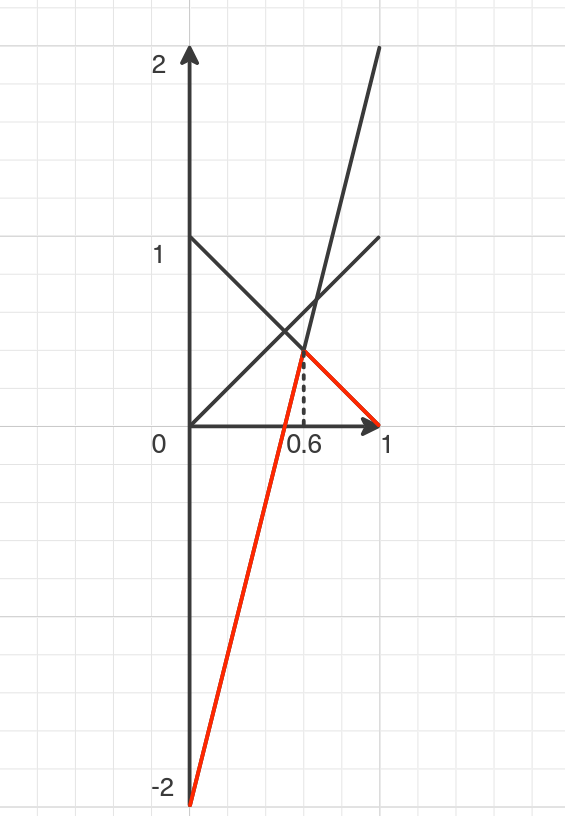
\includegraphics[width=10cm]{image.png}
\end{center}

Строим графики на $[0, 1]$ и ищем максимум нижней огибающей (красная ломаная).
Пересечение $1-p$ и $4p-2$: \\
$1 - p = 4p - 2 \implies p = 0.6$. В этой точке значение равно $0.4$\\
Линия $p$ в точке $p=0.6$ дает $0.6 > 0.4$. Максимум нижней огибающей достигается при $p = 0.6$, цена игры $v = 0.4$.

Активные стратегии 2-го игрока (1-й и 2-й столбцы): \\
$Q = (q, 1-q, 0)$ \\
$0 q + 2(1-q) = 1q - 2(1-q) \implies 2 - 2q = 3q - 2 \implies q = 0.8$.

\textbf{Ответ:} \\
$P = (0.6; 0.4; 0; 0)$ \\
$Q = (0.8; 0.2; 0; 0)$ \\
$v = 0.4$ 


\newpage


% --- ЗАДАНИЕ 6 ---
\section*{Задание 6. Решить матричную игру сведя ее к задача линейного програмиирования}
$$A = \begin{pmatrix} -4 & 4 & 3 \\ -1 & -1 & 2 \\ 4 & -4 & 3 \end{pmatrix}$$

Чтобы использовать симплекс-метод, цена игры должна быть строго положительной. Прибавим ко всем элементам матрицы константу $C = 5$:
$$ A' = A + 5 = \begin{pmatrix} 1 & 9 & 8 \\ 4 & 4 & 7 \\ 9 & 1 & 8 \end{pmatrix} $$
Новая цена игры: $v' = v + C = v + 5$.

Введем переменные: $x_i = \frac{p_i}{v'}$ (для 1-го игрока) и $y_j = \frac{q_j}{v'}$ (для 2-го игрока).

\textbf{Прямая задача (для 1-го игрока):}
$$ F(x) = x_1 + x_2 + x_3 \rightarrow \min $$
при ограничениях:
$$ \begin{cases} 
1x_1 + 4x_2 + 9x_3 \ge 1 \\ 
9x_1 + 4x_2 + 1x_3 \ge 1 \\ 
8x_1 + 7x_2 + 8x_3 \ge 1 \\
x_1 \ge 0, \ x_2 \ge 0, \ x_3 \ge 0
\end{cases} $$

\textbf{Двойственная задача (для 2-го игрока):}
$$ Z(y) = y_1 + y_2 + y_3 \rightarrow \max $$
при ограничениях:
$$ \begin{cases} 
1y_1 + 9y_2 + 8y_3 \le 1 \\ 
4y_1 + 4y_2 + 7y_3 \le 1 \\ 
9y_1 + 1y_2 + 8y_3 \le 1 \\
y_1 \ge 0, \ y_2 \ge 0, \ y_3 \ge 0
\end{cases} $$

Перейдем к канонической форме, добавив балансовые переменные $y_4, y_5, y_6 \ge 0$:
$$ \begin{cases} 
1y_1 + 9y_2 + 8y_3 + y_4 = 1 \\ 
4y_1 + 4y_2 + 7y_3 + y_5 = 1 \\ 
9y_1 + 1y_2 + 8y_3 + y_6 = 1 
\end{cases} $$
Функция цели: $Z - y_1 - y_2 - y_3 = 0$.

\vspace{0.5cm}
Разрешающий столбец: $y_1$ (выбираем любой отрицательный элемент в строке $Z$).\\
Разрешающая строка: $y_6$ (так как $\min(1/1, 1/4, 1/9) = 1/9$).\\
Разрешающий элемент: \textbf{9}

\begin{center}
\renewcommand{\arraystretch}{1.2}
\begin{tabular}{|c|c|c|c|c|c|c|c|}
\hline
Базис & $B$ & $y_1$ & $y_2$ & $y_3$ & $y_4$ & $y_5$ & $y_6$ \\ \hline
$y_4$ & $1$ & $1$ & $9$ & $8$ & $1$ & $0$ & $0$ \\ \hline
$y_5$ & $1$ & $4$ & $4$ & $7$ & $0$ & $1$ & $0$ \\ \hline
$y_6$ & $1$ & \textbf{9} & $1$ & $8$ & $0$ & $0$ & $1$ \\ \hline
$Z$   & $0$ & $-1$& $-1$& $-1$& $0$ & $0$ & $0$ \\ \hline
\end{tabular}
\end{center}

\vspace{0.5cm}
Разрешающий столбец: $y_2$ (так как $-8/9 < 0$).\\
Разрешающая строка: $y_4$ (так как $\min(\frac{8/9}{80/9}, \frac{5/9}{32/9}) = 1/10$).\\
Разрешающий элемент: \textbf{80/9}

\begin{center}
\renewcommand{\arraystretch}{1.8}
\begin{tabular}{|c|c|c|c|c|c|c|c|}
\hline
Базис & $B$ & $y_1$ & $y_2$ & $y_3$ & $y_4$ & $y_5$ & $y_6$ \\ \hline
$y_4$ & $8/9$ & $0$ & \textbf{80/9} & $64/9$ & $1$ & $0$ & $-1/9$ \\ \hline
$y_5$ & $5/9$ & $0$ & $32/9$ & $31/9$ & $0$ & $1$ & $-4/9$ \\ \hline
$y_1$ & $1/9$ & $1$ & $1/9$  & $8/9$  & $0$ & $0$ & $1/9$  \\ \hline
$Z$   & $1/9$ & $0$ & $-8/9$ & $-1/9$ & $0$ & $0$ & $1/9$  \\ \hline
\end{tabular}
\end{center}

\vspace{0.5cm}
Все коэффициенты в индексной строке $Z \ge 0$

\begin{center}
\renewcommand{\arraystretch}{1.8}
\begin{tabular}{|c|c|c|c|c|c|c|c|}
\hline
Базис & $B$ & $y_1$ & $y_2$ & $y_3$ & $y_4$ & $y_5$ & $y_6$ \\ \hline
$y_2$ & $1/10$ & $0$ & $1$ & $4/5$ & $9/80$ & $0$ & $-1/80$\\ \hline
$y_5$ & $1/5$  & $0$ & $0$ & $3/5$ & $-2/5$ & $1$ & $-2/5$ \\ \hline
$y_1$ & $1/10$ & $1$ & $0$ & $4/5$ & $-1/80$& $0$ & $9/80$ \\ \hline
$Z$   & $1/5$  & $0$ & $0$ & $3/5$ & $1/10$ & $0$ & $1/10$ \\ \hline
\end{tabular}
\end{center}

\vspace{0.5cm}
\textbf{Вывод ответа}\\
Из столбца $B$ последней таблицы выписываем равновесное решение для Второго игрока:
$$Z_{\max} = \frac{1}{5}, \quad y_1 = \frac{1}{10}, \quad y_2 = \frac{1}{10}, \quad y_3 = 0$$

Находим новую и исходную цену игры:
$$v' = \frac{1}{Z_{\max}} = 5 \implies v = v' - C = 5 - 5 = 0$$

\textbf{Стратегии Второго игрока ($Q$):}\\
По формуле $q_j = y_j \cdot v'$:
$$q_1 = \frac{1}{10} \cdot 5 = \frac{1}{2}, \quad q_2 = \frac{1}{10} \cdot 5 = \frac{1}{2}, \quad q_3 = 0 \cdot 5 = 0$$
Равновесная стратегия: $S_2^* = \left(\frac{1}{2}; \frac{1}{2}; 0\right)$.

\vspace{0.5cm}
Равновесное решение для Первого игрока берем из индексной строки $Z$ под балансовыми переменными $y_4, y_5, y_6$:
$$x_1 = Z_{y_4} = \frac{1}{10}, \quad x_2 = Z_{y_5} = 0, \quad x_3 = Z_{y_6} = \frac{1}{10}$$

\textbf{Стратегии Первого игрока ($P$):}\\
По формуле $p_i = x_i \cdot v'$:
$$p_1 = \frac{1}{10} \cdot 5 = \frac{1}{2}, \quad p_2 = 0 \cdot 5 = 0, \quad p_3 = \frac{1}{10} \cdot 5 = \frac{1}{2}$$
Равновесное стратегия: $S_1^* = \left(\frac{1}{2}; 0; \frac{1}{2}\right)$.

\vspace{0.5cm}
\textbf{Ответ:}
\begin{itemize}
    \item Цена игры: $v = 0$
    \item Равновесная стратегия 1-го игрока: $S_1^* = \left(\frac{1}{2}; 0; \frac{1}{2}\right)$
    \item Равновесная стратегия 2-го игрока: $S_2^* = \left(\frac{1}{2}; \frac{1}{2}; 0\right)$
\end{itemize}


\newpage


% --- ЗАДАНИЕ 7 ---
\section*{Задание 7. Определить все значения параметра, при котором в игре есть седловая точка}
$$A = \begin{pmatrix} 3 & a \\ a & 1 \end{pmatrix}$$
Седловая точка существует, если максимин равен минимаксу ($\underbar{v} = \bar{\text{v}}$)
\begin{itemize}
    \item Нижняя цена: $\underbar{v} = \max(\min(3, a), \min(a, 1))$
    \item Верхняя цена: $\bar{\text{v}} = \min(\max(3, a), \max(a, 1))$
\end{itemize}

Рассмотрим интервал $a < 1$: \\
$\underbar{v} = \max(1, a) = 1$, $\bar{\text{v}} = \min(3, a) = a$. Условие $\underbar{v} = \bar{\text{v}}$ не выполняется \\

Рассмотрим интервал $1 \le a \le 3$: \\
$\underbar{v} = \max(1, a) = a$, $\bar{\text{v}} = \min(3, a) = a$. Условие $\underbar{v} = \bar{\text{v}}$ выполняется \\

Рассмотрим интервал $3 < a$: \\
$\underbar{v} = \max(1, a) = a$, $\bar{\text{v}} = \min(3, a) = 3$. Условие $\underbar{v} = \bar{\text{v}}$ не выполняется \\

\textbf{Ответ:} $a \in [1; 3]$.


\newpage


% --- ЗАДАНИЕ 8 ---
\section*{Задание 8. Решить биматричную игру}
$$A = \begin{pmatrix} 2 & 0 \\ 0 & 1 \end{pmatrix}, \quad B = \begin{pmatrix} 1 & 0 \\ 0 & 2 \end{pmatrix}$$ \\

Матрица исходов: $M = \begin{pmatrix} (2, 1) & (0, 0) \\ (0, 0) & (1, 2) \end{pmatrix}$ \\

\subsection*{Равновесие по Нэшу (в чистых стратегиях):}
Лучшие ответы игроков совпадают в клетках $(R_1, C_1)$ и $(R_2, C_2)$.
Следовательно, чистые равновесия Нэша — профили (1-я, 1-я) и (2-я, 2-я).

\subsection*{Равновесие по Нэшу (в смешанных стратегиях):}
Пусть $P=(p, 1-p)$, $Q=(q, 1-q)$ \\
Игрок 1: $2q = 1(1-q) \implies 3q = 1 \implies q = \frac{1}{3}$ \\
Игрок 2: $1p = 2(1-p) \implies 3p = 2 \implies p = \frac{2}{3}$ \\
Смешанное равновесие: $P = (\frac{2}{3}, \frac{1}{3})$, $Q = (\frac{1}{3}, \frac{2}{3})$

\subsection*{Оптимальность по Парето:}
\begin{itemize}
    \item Исход $(0, 0)$ не оптимален (хуже обоих других исходов)
    \item Исходы $(2, 1)$ и $(1, 2)$ являются оптимальными по Парето, так как невозможно улучшить выигрыш одного игрока, не ухудшив выигрыш другого
\end{itemize}

\textbf{Ответ:} 
Равновесия Нэша: (1, 1), (2, 2) и смешанное $P=(\frac{2}{3}, \frac{1}{3}), Q=(\frac{1}{3}, \frac{2}{3})$.
Оптимальные по Парето исходы: (1-я строка, 1-й столбец) и (2-я строка, 2-й столбец).




\end{document}